\subsection{\label{sec:label2}The INGRID geometry collection}
If we are to adopt an object-oriented approach to grid generation, then we must develop a set of tools that can be utilized throughout our project. Here we discuss how INGRID defines a collection of geometric classes in order to make the grid generating process as simple as possible for all magnetic topologies of interest. To do so, INGRID defines the following collection of geometric abstractions: the Point class, the Line class, the Cell class, and the Patch class. All together, these classes arm INGRID with the ability to represent any magnetic topology of interest. We provide a very brief description of the classes here. Figure \ref{fig:geo_collection} illustrates the geometry collection described below.\\
\begin{figure}
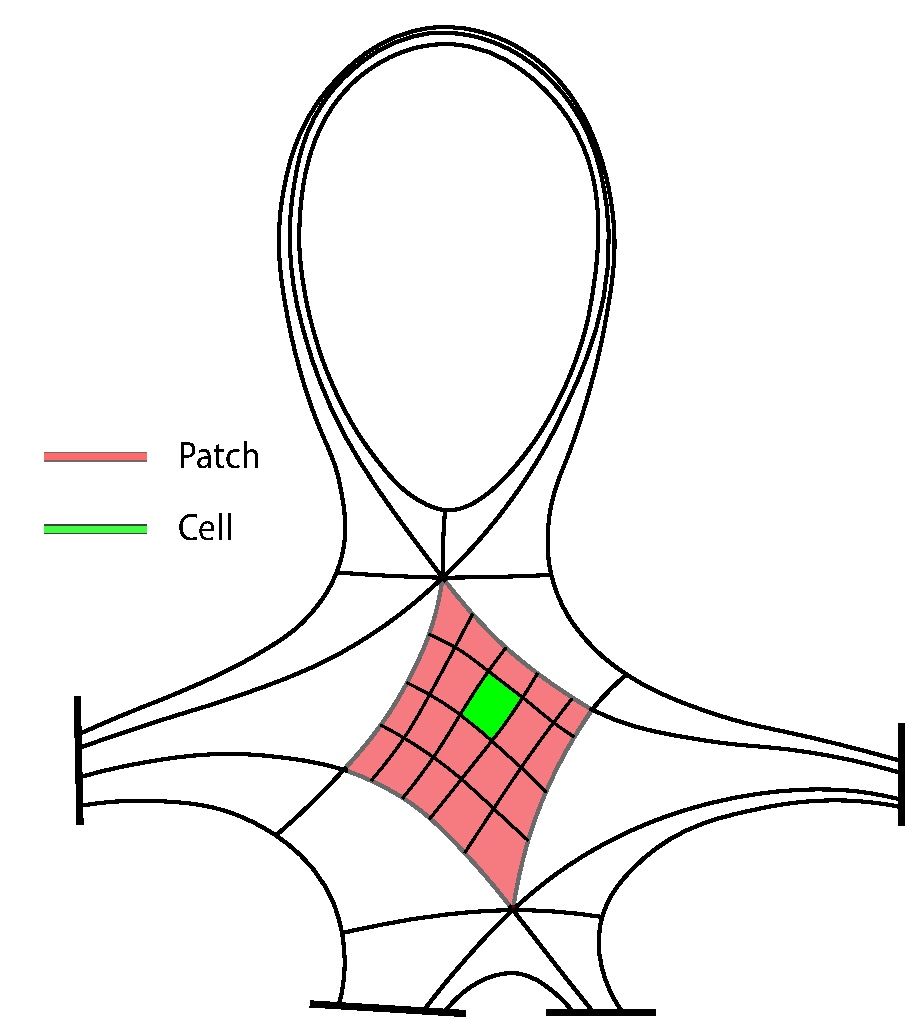
\includegraphics[scale=0.35]{figures/geometry_render.pdf}  % scale=0.35
\caption{\label{fig:geo_collection} INGRID geometric objects are used to represent an arbitrary magnetic topology. Here we explicitly see a Patch, Cell, and Line. Points are implicitly shown by a Line and Cell object definition.}
\end{figure}
\indent
A Point object simply represents an arbitrary $(r,z)$ spatial coordinate. A Line object object is defined by two or more Point objects. This Line object definition allows for the representation of any arbitrary curve we may encounter (e.g. psi-surface, target plate, limiter geometry). A Patch object represents a quadrilateral region of the domain. Patches are defined by four Line objects. This Patch abstraction allows for partitioning of the domain of interest into various regions that we would like to obtain a grid representation of. A Cell object resides within a Patch and represents a quadrilateral grid cell. Cells are defined by five Point objects: four corners and a center. These Cell objects contain spatial and experimental data that are to be used in simulation code.\\ \indent
From these definitions, we have the building blocks for modeling any of the magnetic topologies of interest we mentioned in the previous section and shown in figure \ref{fig:config_group}. In particular, we aim to construct a collection of Patch objects representing the divertor configuration of interest. We call this collection of Patch objects a Patch map. This Patch map allows us to create a grid of Cell objects within each Patch, thus providing the final grid. We illustrate the idea in figure \ref{fig:snl_patch_index_space} by showing the relation between an SNL Patch map and the corresponding grid in index space. The management of the Patch map creation and grid generation is managed by a magnetic topology class of modeling interest. \\ \indent
As of the current INGRID release, we have defined magnetic topology classes SNL, UDN, SF15, SF45, SF75, SF105, SF135, and SF165. These are contained within a dedicated topologies subpackage within the INGRID code. We also introduce a general ``Ingrid" class exclusively meant for user interfacing and management. The Ingrid class and all magnetic topologies are supported by the backend utility classes IngridUtils and TopologyUtils respectively. We will discuss these classes at a later part of the report.
\begin{figure}
    \centering
    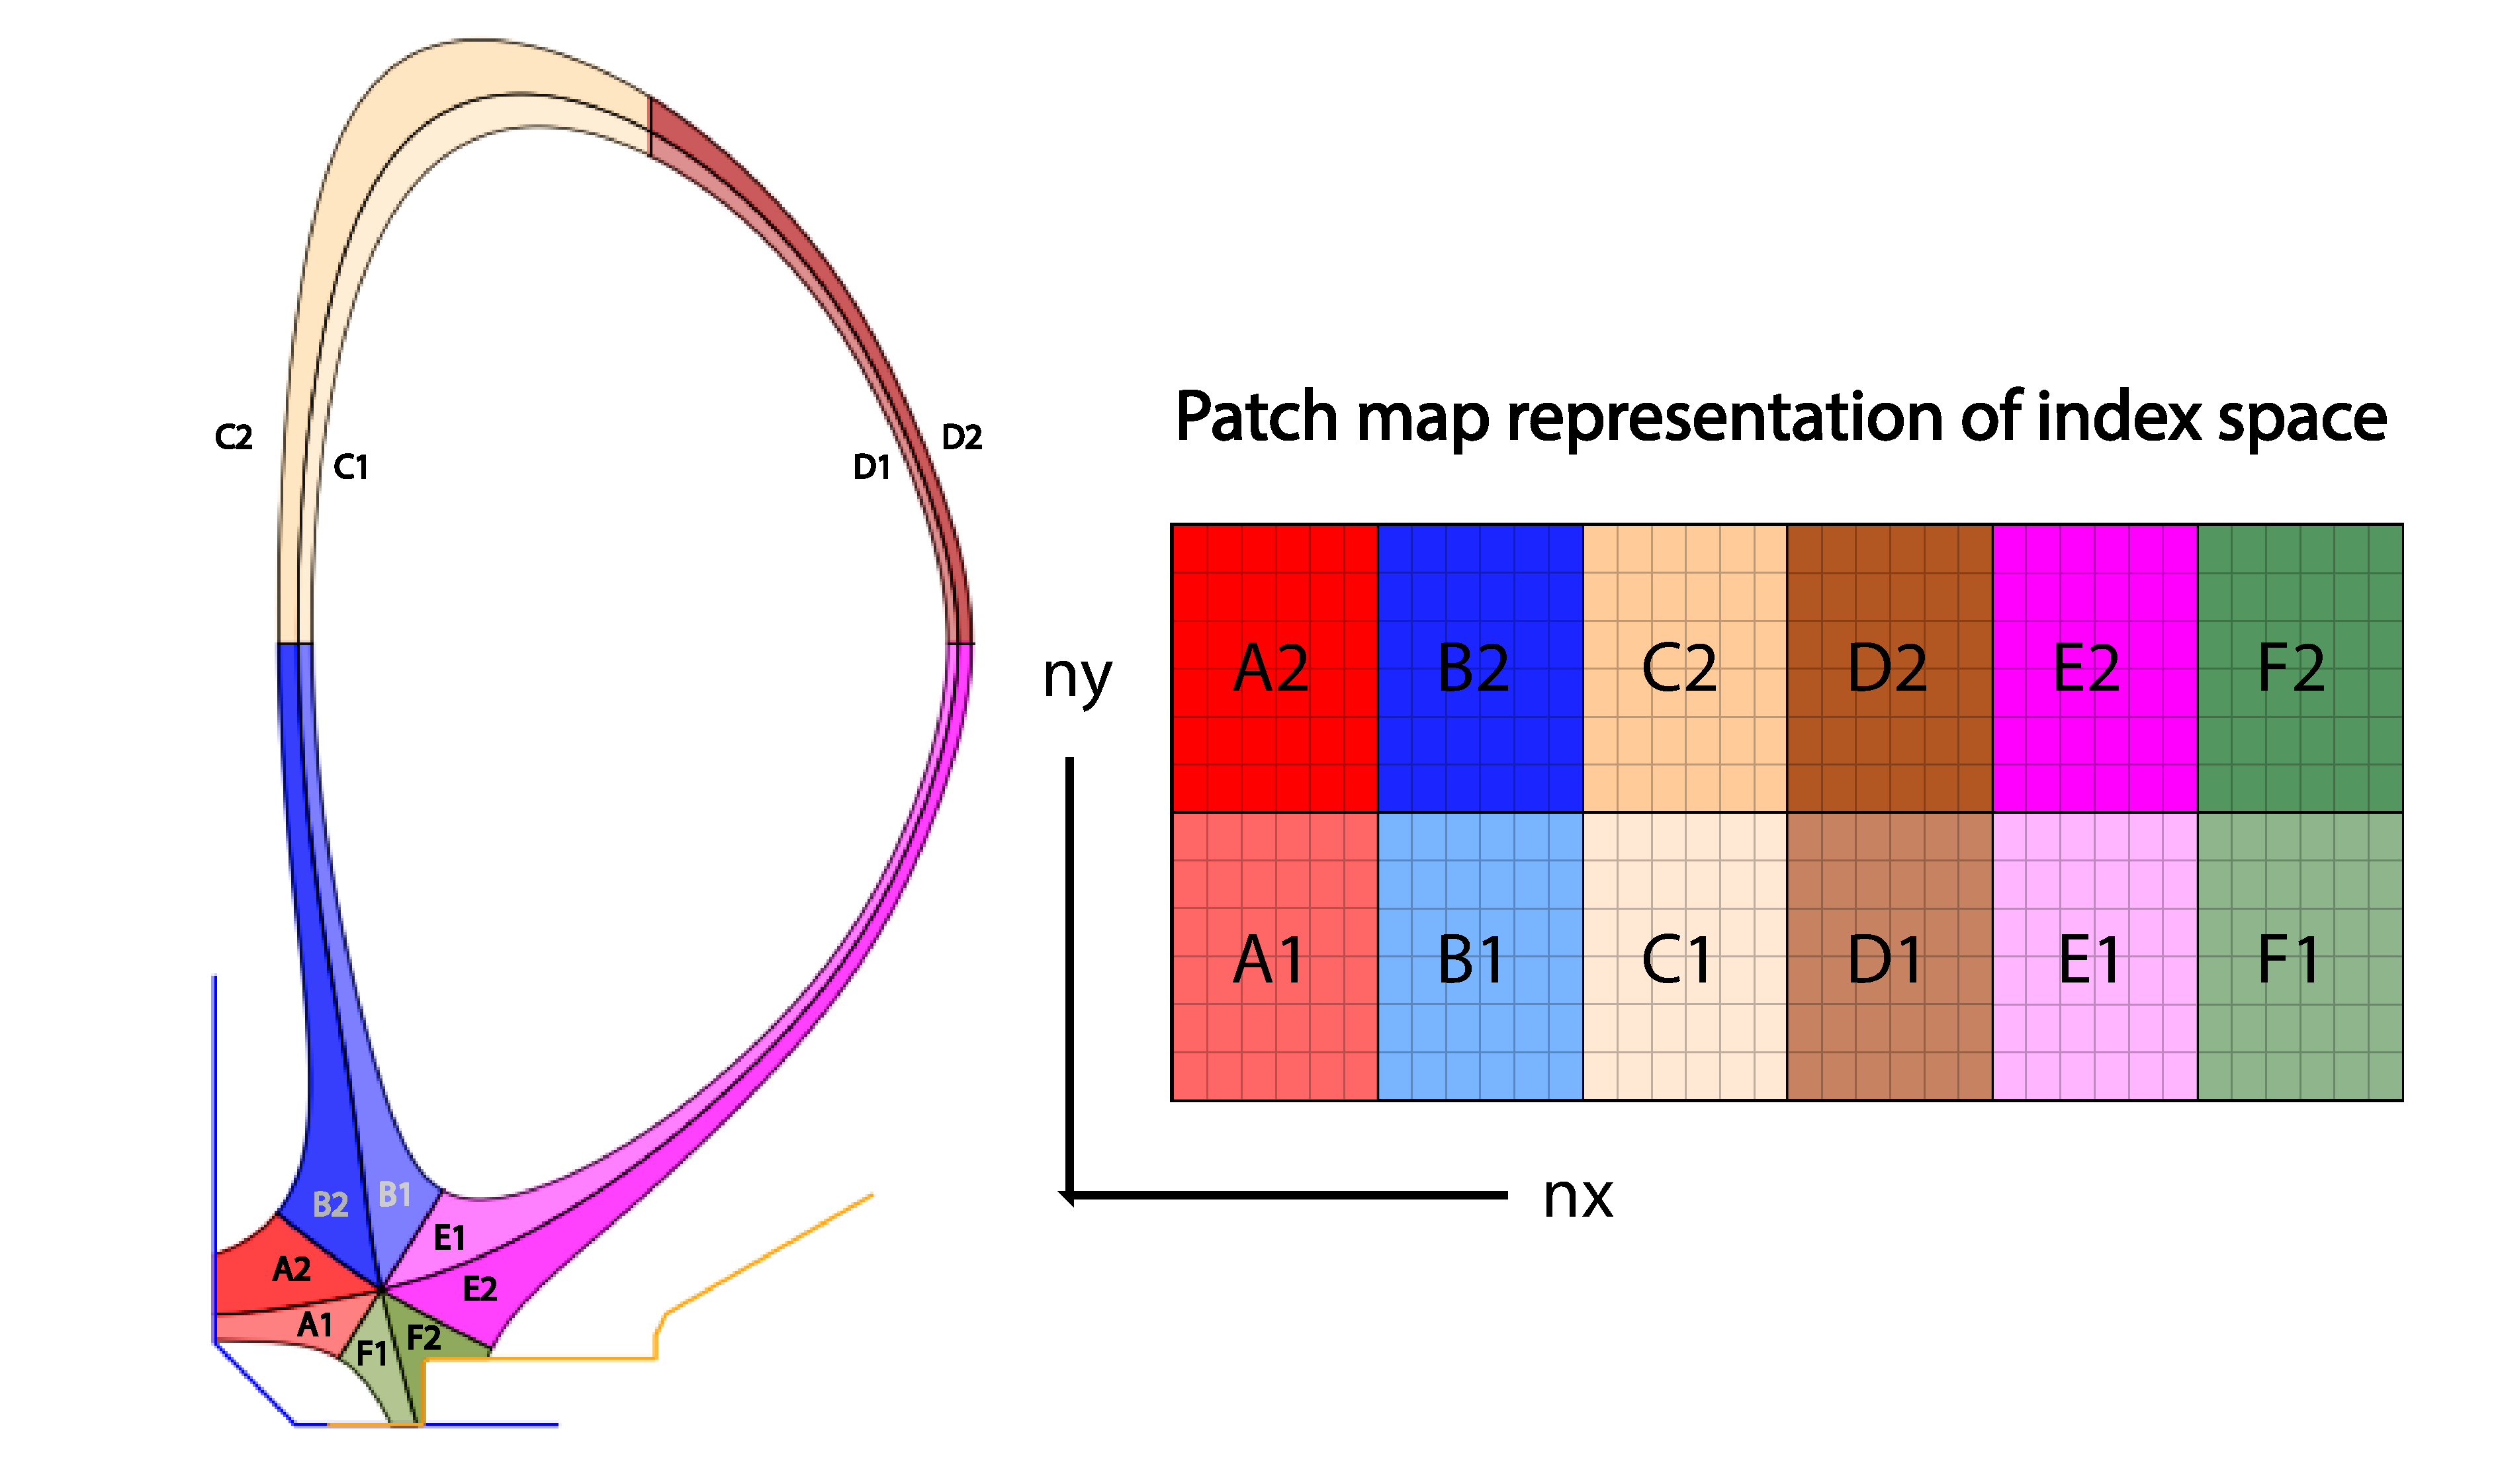
\includegraphics[width=\linewidth]{figures/patch_index_space.pdf}
    \caption{The Patch map of an SNL configuration and it's correspondence to a grid in index space. Individual Patch objects and their region in index space are labeled with a two-character key.}
    \label{fig:snl_patch_index_space}
\end{figure}